\newpage
\section{Tinjauan Pustaka}

\subsection{Customer Churn}
% Buat tinjauan pustaka untuk Customer churn gunakan refrensi yang relevan
Customer churn, atau kehilangan pelanggan, adalah fenomena di mana pelanggan berhenti menggunakan layanan atau produk yang ditawarkan oleh suatu perusahaan. Hal ini menjadi perhatian utama bagi perusahaan, terutama di industri yang sangat kompetitif seperti telekomunikasi, karena churn dapat berdampak langsung pada pendapatan dan profitabilitas.

\subsection{EDA (Exploratory Data Analysis)}
% Buat tinjauan pustaka untuk EDA gunakan refrensi yang relevan
Exploratory Data Analysis (EDA) adalah proses analisis data yang bertujuan untuk memahami struktur, pola, dan hubungan dalam dataset sebelum menerapkan model statistik atau machine learning. EDA melibatkan visualisasi data, statistik deskriptif, dan identifikasi anomali atau outlier. Proses ini penting untuk mendapatkan wawasan awal tentang data dan membantu dalam pengambilan keputusan selanjutnya.

\subsection{Model Klasifikasi}
% Buat tinjauan pustaka untuk Model Klasifikasi gunakan refrensi yang relevan
Model klasifikasi adalah teknik dalam machine learning yang digunakan untuk mengelompokkan data ke dalam kategori atau kelas tertentu. Model ini dilatih menggunakan dataset yang berisi fitur-fitur input dan label output yang sesuai. Tujuan dari model klasifikasi adalah untuk memprediksi kelas dari data baru berdasarkan pola yang telah dipelajari dari data pelatihan.

\subsection{Logistic Regression}
% Buat tinjauan pustaka untuk Logistic Regression gunakan refrensi yang relevan
Logistic regression adalah metode statistik yang digunakan untuk analisis regresi ketika variabel dependen bersifat kategorikal. Meskipun namanya mengandung kata "regression", logistic regression sebenarnya digunakan untuk klasifikasi. Metode ini memodelkan probabilitas suatu kejadian dengan menggunakan fungsi logit, yang mengubah output linear menjadi nilai antara 0 dan 1, sehingga cocok untuk prediksi kelas biner.

Untuk memahami logistic regression, kita perlu memahami konsep dasar dari regresi logistik. Regresi logistik digunakan untuk memprediksi probabilitas dari suatu kejadian yang bersifat biner (dua kelas), seperti churn atau tidak churn. Model ini mengasumsikan bahwa log odds dari probabilitas kejadian tersebut adalah linear terhadap fitur-fitur input.

%masukan rumus logistic regression untuk pemodelan
\begin{equation}
    P(Y=1|X) = \frac{1}{1 + e^{-(\beta_0 + \beta_1 X_1 + \beta_2 X_2 + ... + \beta_n X_n)}}
\end{equation}

di mana:
\begin{itemize}
    \item \( P(Y=1|X) \) adalah probabilitas bahwa kelas target \( Y \) adalah 1 (misalnya, churn).
    \item \( \beta_0 \) adalah intercept dari model.
    \item \( \beta_1, \beta_2, ..., \beta_n \) adalah koefisien regresi untuk fitur \( X_1, X_2, ..., X_n \).
    \item \( e \) adalah basis dari logaritma natural.
    \item \( X_1, X_2, ..., X_n \) adalah fitur-fitur input yang digunakan untuk memprediksi kelas target.
\end{itemize}

Dalam tugas ini apabila perhitungan probabilitas P(Y=1|X) lebih besar dari 0.5 maka akan dikategorikan sebagai churn, sebaliknya jika kurang dari 0.5 maka tidak churn.

\subsection{Random Forest}
% Buat tinjauan pustaka untuk Random Forest gunakan refrensi yang relevan
Random Forest adalah algoritma ensemble learning yang menggabungkan beberapa pohon keputusan (decision trees) untuk meningkatkan akurasi prediksi. Setiap pohon dalam hutan dibangun menggunakan subset acak dari data pelatihan dan fitur, sehingga mengurangi risiko overfitting yang sering terjadi pada pohon keputusan tunggal. Random Forest dapat digunakan untuk klasifikasi maupun regresi, dan memiliki keunggulan dalam menangani data besar dengan banyak fitur.

%masukan rumus random forest untuk pemodelan
\begin{equation}
    \hat{Y} = \frac{1}{N} \sum_{i=1}^{N} T_i(X)
\end{equation}
di mana:
\begin{itemize}
    \item \( \hat{Y} \) adalah prediksi akhir dari Random Forest.
    \item \( N \) adalah jumlah pohon dalam hutan.
    \item \( T_i(X) \) adalah prediksi dari pohon keputusan ke-i untuk input \( X \).
    \item \( X \) adalah fitur-fitur input yang digunakan untuk memprediksi kelas target.
    \item \( \sum_{i=1}^{N} T_i(X) \) adalah jumlah prediksi dari semua pohon dalam hutan.
\end{itemize}

\subsection{XGBoost/Gradient Boosting}
% Buat tinjauan pustaka untuk XGBoost/Gradient Boosting gunakan refrensi yang relevan
XGBoost (Extreme Gradient Boosting) adalah algoritma machine learning yang merupakan implementasi dari teknik gradient boosting. XGBoost dirancang untuk efisiensi, fleksibilitas, dan kinerja yang tinggi. Algoritma ini membangun model prediksi secara bertahap dengan menambahkan pohon keputusan baru yang mengoreksi kesalahan dari pohon sebelumnya. XGBoost sangat populer dalam kompetisi data science karena kemampuannya dalam menangani data besar dan kompleks.
%masukan rumus XGBoost untuk pemodelan
\begin{equation}
    \hat{y}_i = \sum_{k=1}^{K} f_k(x_i)
\end{equation}
di mana:
\begin{itemize}
    \item \( \hat{y}_i \) adalah prediksi untuk data ke-i.
    \item \( K \) adalah jumlah pohon dalam model XGBoost.
    \item \( f_k(x_i) \) adalah output dari pohon ke-k untuk input \( x_i \).
    \item \( x_i \) adalah fitur-fitur input yang digunakan untuk memprediksi kelas target.
    \item \( \sum_{k=1}^{K} f_k(x_i) \) adalah jumlah prediksi dari semua pohon dalam model XGBoost.
\end{itemize}

\subsection{Confusion Matrix}
% Buat tinjauan pustaka untuk Confusion Matrix gunakan refrensi yang relevan
\emph{Confusion matrix} merupakan salah satu pengukuran yang paling mudah dilakukan dalam mencari nilai tingkat kebenaran dan juga akurasi dari model. \emph{Confusion matrix} adalah sebuah tabel berbentuk dua dimensi yang terdiri dari data aktual dan data prediksi yang masing-masing memiliki kelas. Data aktual terletak pada bagian kolom tabel, sedangkan data prediksi terletak pada bagian baris dari tabel. Gambar \ref{fig:confusion_matrix} merupakan representasi visual dari perhitungan confusion matrix.

\begin{figure}[ht]
    \centering
    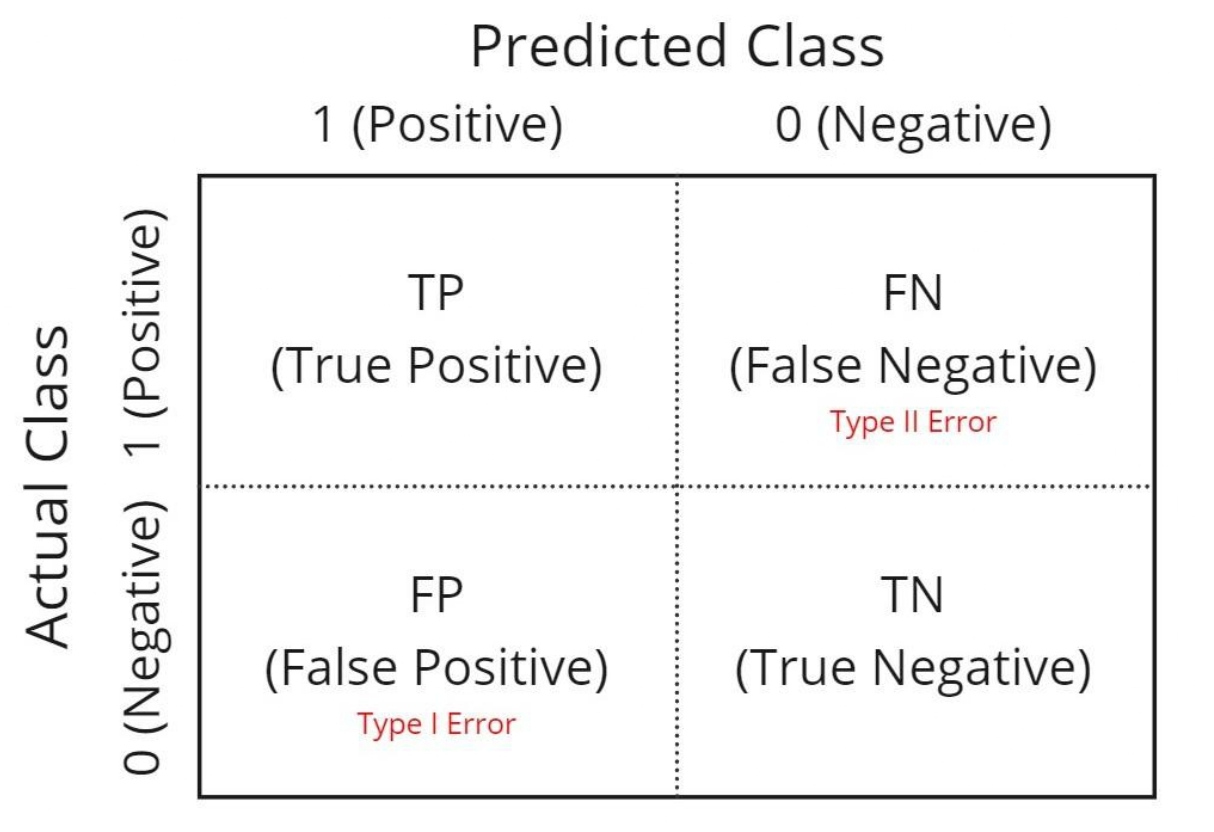
\includegraphics[width=0.5\textwidth]{gambar/conf.jpg}
    \caption{Contoh Confusion Matrix}
    \label{fig:confusion_matrix}
\end{figure}

Confusion matrix memberikan informasi tentang jumlah prediksi yang benar dan salah untuk setiap kelas. Dari confusion matrix, kita dapat menghitung berbagai metrik evaluasi model seperti akurasi, presisi, recall, dan F1-score. Metrik-metrik ini membantu dalam menilai kinerja model klasifikasi secara keseluruhan.

\subsection{Recall}
% Buat tinjauan pustaka untuk Recall gunakan refrensi yang relevan
Recall, juga dikenal sebagai sensitivitas atau true positive rate, adalah metrik evaluasi yang mengukur kemampuan model dalam mengidentifikasi kelas positif. Recall didefinisikan sebagai rasio antara jumlah prediksi benar positif (true positives) dengan jumlah total kasus positif aktual (true positives + false negatives). Rumusnya adalah:

\begin{equation}
    \text{Recall} = \frac{\text{True Positives}}{\text{True Positives} + \text{False Negatives}}
\end{equation}

di mana:
\begin{itemize}
    \item True Positives (TP): Jumlah kasus positif yang benar-benar terdeteksi oleh model.
    \item False Negatives (FN): Jumlah kasus positif yang tidak terdeteksi oleh model (salah diklasifikasikan sebagai negatif).
\end{itemize}

Recall sangat penting dalam konteks di mana kita ingin meminimalkan jumlah kasus positif yang terlewatkan, seperti dalam deteksi penyakit atau pencegahan churn pelanggan. Metrik ini memberikan gambaran tentang seberapa baik model dapat menangkap semua kasus positif yang sebenarnya ada.

\subsection{ROC-AUC}
% Buat tinjauan pustaka untuk ROC-AUC gunakan refrensi yang relevan
ROC (Receiver Operating Characteristic) curve adalah grafik yang menunjukkan kinerja model klasifikasi biner pada berbagai ambang batas (threshold). ROC curve memplot true positive rate (TPR) terhadap false positive rate (FPR) pada berbagai nilai threshold. Area di bawah kurva ROC (AUC - Area Under the Curve) memberikan ukuran kinerja model secara keseluruhan.

AUC adalah nilai antara 0 dan 1, di mana nilai 1 menunjukkan model yang sempurna (mampu memisahkan kelas positif dan negatif dengan sempurna), sedangkan nilai 0.5 menunjukkan model yang tidak lebih baik dari tebakan acak. AUC yang lebih tinggi menunjukkan bahwa model memiliki kemampuan yang lebih baik dalam membedakan antara kelas positif dan negatif.

\begin{equation}
    \text{AUC} = \int_0^1 \text{TPR}(FPR) \, dFPR
\end{equation}

di mana:
\begin{itemize}
    \item TPR (True Positive Rate) adalah rasio antara jumlah prediksi benar positif dengan jumlah total kasus positif aktual.
    \item FPR (False Positive Rate) adalah rasio antara jumlah prediksi salah positif dengan jumlah total kasus negatif aktual.
    \item Integral ini menghitung area di bawah kurva ROC, yang memberikan nilai AUC.
    \item Nilai AUC yang lebih tinggi menunjukkan bahwa model memiliki kemampuan yang lebih baik dalam membedakan antara kelas positif dan negatif.
\end{itemize}